% V-model -- include with % V-model -- include with % V-model -- include with % V-model -- include with \input{chapters/vmodel}
% Needs only TikZ + the positioning library (already loaded via forest in main.tex)
\begin{figure}[H]
  \centering
  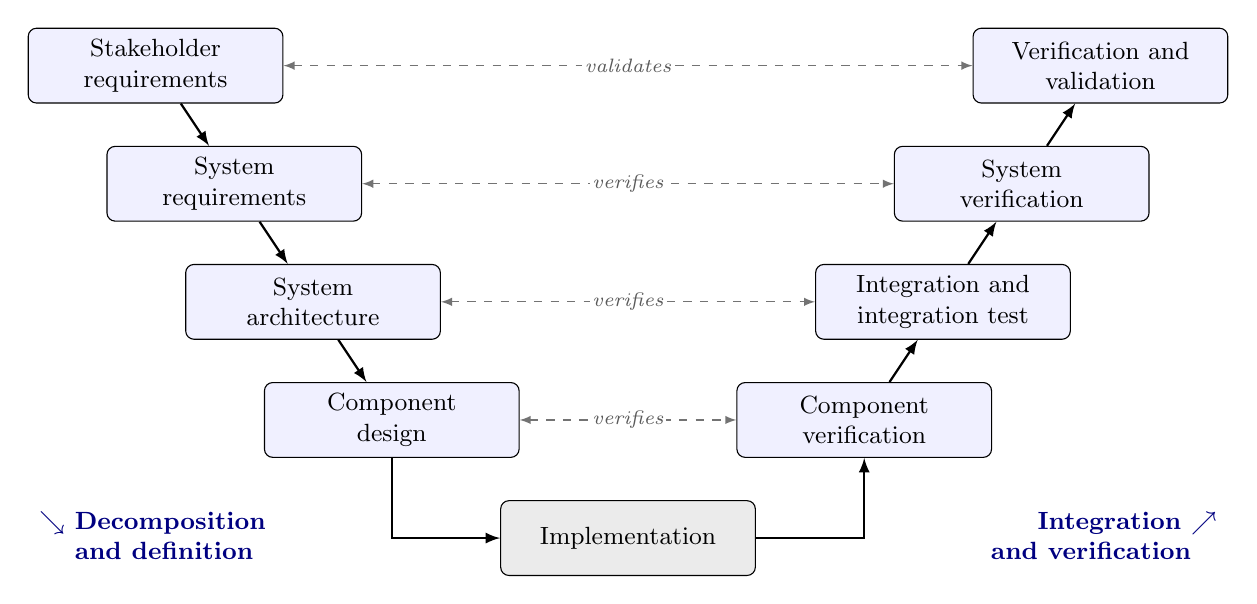
\begin{tikzpicture}[
      >=latex,
      font=\small,
      phase/.style={draw, rounded corners=3pt, fill=blue!6, align=center,
                    minimum width=3.2cm, minimum height=0.95cm, text width=3.0cm},
      impl/.style ={phase, fill=black!8},
      flow/.style ={->, thick},
      link/.style ={<->, dashed, black!55},
      lbl/.style  ={font=\scriptsize\itshape, text=black!65, fill=white, inner sep=1pt},
    ]
    % Left branch: specification and design (top to bottom)
    \node[phase] (req)  at (0.0, 0.0)  {Stakeholder\\requirements};
    \node[phase] (sys)  at (1.0,-1.5)  {System\\requirements};
    \node[phase] (arch) at (2.0,-3.0)  {System\\architecture};
    \node[phase] (comp) at (3.0,-4.5)  {Component\\design};

    % Bottom
    \node[impl]  (impl) at (6.0,-6.0)  {Implementation};

    % Right branch: integration and verification (bottom to top)
    \node[phase] (cver) at (9.0,-4.5)  {Component\\verification};
    \node[phase] (int)  at (10.0,-3.0) {Integration and\\integration test};
    \node[phase] (sver) at (11.0,-1.5) {System\\verification};
    \node[phase] (val)  at (12.0, 0.0) {Verification and\\validation};

    % Process flow along the V
    \draw[flow] (req)  -- (sys);
    \draw[flow] (sys)  -- (arch);
    \draw[flow] (arch) -- (comp);
    \draw[flow] (comp) |- (impl);
    \draw[flow] (impl) -| (cver);
    \draw[flow] (cver) -- (int);
    \draw[flow] (int)  -- (sver);
    \draw[flow] (sver) -- (val);

    % Verification / validation relationships across the V
    \draw[link] (req.east)  -- node[lbl] {validates} (val.west);
    \draw[link] (sys.east)  -- node[lbl] {verifies}  (sver.west);
    \draw[link] (arch.east) -- node[lbl] {verifies}  (int.west);
    \draw[link] (comp.east) -- node[lbl] {verifies}  (cver.west);

    % Branch labels (bottom corners, outside the V)
    \node[font=\small\bfseries, text=blue!50!black, align=left, anchor=west]
      at (-1.6,-6.0) {$\searrow$ Decomposition\\\phantom{$\searrow$} and definition};
    \node[font=\small\bfseries, text=blue!50!black, align=right, anchor=east]
      at (13.6,-6.0) {Integration $\nearrow$\\and verification\phantom{$\nearrow$}};
  \end{tikzpicture}

  \caption[V-model of the system development process]{%
    V-model of the system development process. The left branch decomposes
    stakeholder requirements step by step into system requirements, an
    architecture and component designs; after implementation, the right
    branch integrates the components into the complete system. Each
    level on the right is verified against its counterpart on the left
    (dashed arrows), and the finished system is validated against the
    original stakeholder requirements.}
  \label{fig:vmodel}
\end{figure}

% Needs only TikZ + the positioning library (already loaded via forest in main.tex)
\begin{figure}[H]
  \centering
  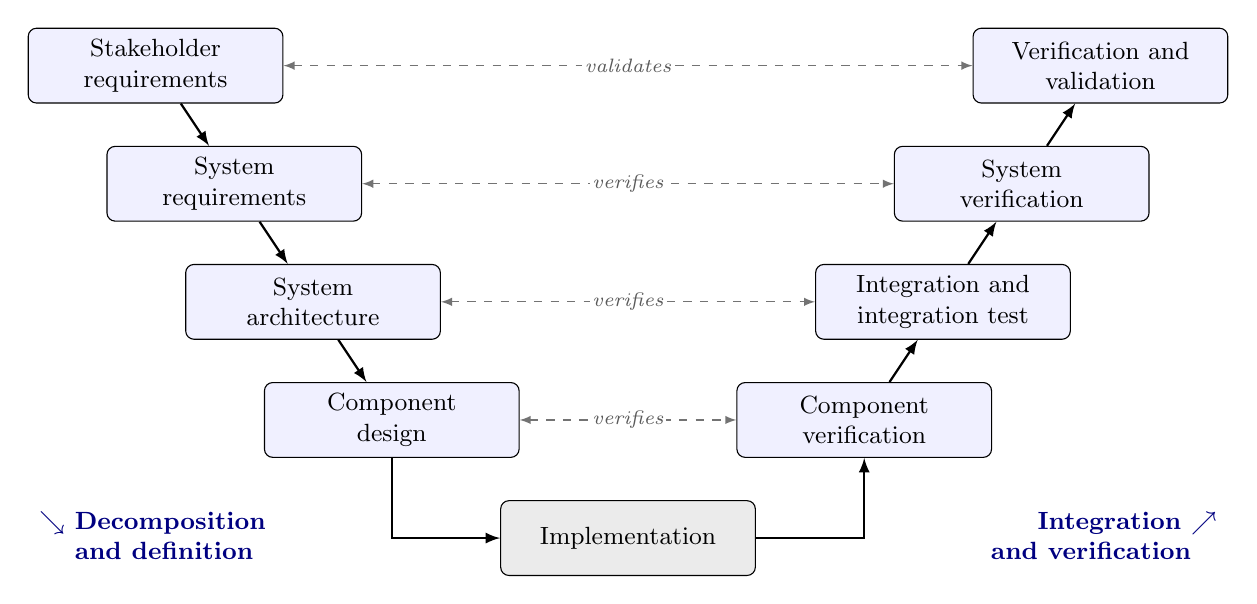
\begin{tikzpicture}[
      >=latex,
      font=\small,
      phase/.style={draw, rounded corners=3pt, fill=blue!6, align=center,
                    minimum width=3.2cm, minimum height=0.95cm, text width=3.0cm},
      impl/.style ={phase, fill=black!8},
      flow/.style ={->, thick},
      link/.style ={<->, dashed, black!55},
      lbl/.style  ={font=\scriptsize\itshape, text=black!65, fill=white, inner sep=1pt},
    ]
    % Left branch: specification and design (top to bottom)
    \node[phase] (req)  at (0.0, 0.0)  {Stakeholder\\requirements};
    \node[phase] (sys)  at (1.0,-1.5)  {System\\requirements};
    \node[phase] (arch) at (2.0,-3.0)  {System\\architecture};
    \node[phase] (comp) at (3.0,-4.5)  {Component\\design};

    % Bottom
    \node[impl]  (impl) at (6.0,-6.0)  {Implementation};

    % Right branch: integration and verification (bottom to top)
    \node[phase] (cver) at (9.0,-4.5)  {Component\\verification};
    \node[phase] (int)  at (10.0,-3.0) {Integration and\\integration test};
    \node[phase] (sver) at (11.0,-1.5) {System\\verification};
    \node[phase] (val)  at (12.0, 0.0) {Verification and\\validation};

    % Process flow along the V
    \draw[flow] (req)  -- (sys);
    \draw[flow] (sys)  -- (arch);
    \draw[flow] (arch) -- (comp);
    \draw[flow] (comp) |- (impl);
    \draw[flow] (impl) -| (cver);
    \draw[flow] (cver) -- (int);
    \draw[flow] (int)  -- (sver);
    \draw[flow] (sver) -- (val);

    % Verification / validation relationships across the V
    \draw[link] (req.east)  -- node[lbl] {validates} (val.west);
    \draw[link] (sys.east)  -- node[lbl] {verifies}  (sver.west);
    \draw[link] (arch.east) -- node[lbl] {verifies}  (int.west);
    \draw[link] (comp.east) -- node[lbl] {verifies}  (cver.west);

    % Branch labels (bottom corners, outside the V)
    \node[font=\small\bfseries, text=blue!50!black, align=left, anchor=west]
      at (-1.6,-6.0) {$\searrow$ Decomposition\\\phantom{$\searrow$} and definition};
    \node[font=\small\bfseries, text=blue!50!black, align=right, anchor=east]
      at (13.6,-6.0) {Integration $\nearrow$\\and verification\phantom{$\nearrow$}};
  \end{tikzpicture}

  \caption[V-model of the system development process]{%
    V-model of the system development process. The left branch decomposes
    stakeholder requirements step by step into system requirements, an
    architecture and component designs; after implementation, the right
    branch integrates the components into the complete system. Each
    level on the right is verified against its counterpart on the left
    (dashed arrows), and the finished system is validated against the
    original stakeholder requirements.}
  \label{fig:vmodel}
\end{figure}

% Needs only TikZ + the positioning library (already loaded via forest in main.tex)
\begin{figure}[H]
  \centering
  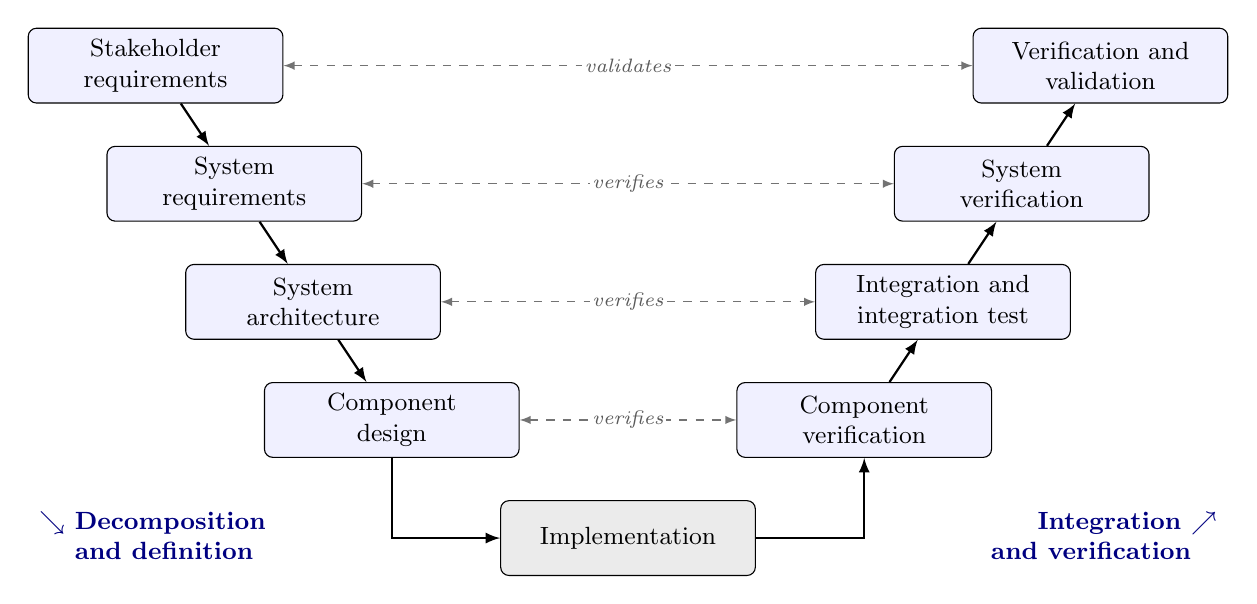
\begin{tikzpicture}[
      >=latex,
      font=\small,
      phase/.style={draw, rounded corners=3pt, fill=blue!6, align=center,
                    minimum width=3.2cm, minimum height=0.95cm, text width=3.0cm},
      impl/.style ={phase, fill=black!8},
      flow/.style ={->, thick},
      link/.style ={<->, dashed, black!55},
      lbl/.style  ={font=\scriptsize\itshape, text=black!65, fill=white, inner sep=1pt},
    ]
    % Left branch: specification and design (top to bottom)
    \node[phase] (req)  at (0.0, 0.0)  {Stakeholder\\requirements};
    \node[phase] (sys)  at (1.0,-1.5)  {System\\requirements};
    \node[phase] (arch) at (2.0,-3.0)  {System\\architecture};
    \node[phase] (comp) at (3.0,-4.5)  {Component\\design};

    % Bottom
    \node[impl]  (impl) at (6.0,-6.0)  {Implementation};

    % Right branch: integration and verification (bottom to top)
    \node[phase] (cver) at (9.0,-4.5)  {Component\\verification};
    \node[phase] (int)  at (10.0,-3.0) {Integration and\\integration test};
    \node[phase] (sver) at (11.0,-1.5) {System\\verification};
    \node[phase] (val)  at (12.0, 0.0) {Verification and\\validation};

    % Process flow along the V
    \draw[flow] (req)  -- (sys);
    \draw[flow] (sys)  -- (arch);
    \draw[flow] (arch) -- (comp);
    \draw[flow] (comp) |- (impl);
    \draw[flow] (impl) -| (cver);
    \draw[flow] (cver) -- (int);
    \draw[flow] (int)  -- (sver);
    \draw[flow] (sver) -- (val);

    % Verification / validation relationships across the V
    \draw[link] (req.east)  -- node[lbl] {validates} (val.west);
    \draw[link] (sys.east)  -- node[lbl] {verifies}  (sver.west);
    \draw[link] (arch.east) -- node[lbl] {verifies}  (int.west);
    \draw[link] (comp.east) -- node[lbl] {verifies}  (cver.west);

    % Branch labels (bottom corners, outside the V)
    \node[font=\small\bfseries, text=blue!50!black, align=left, anchor=west]
      at (-1.6,-6.0) {$\searrow$ Decomposition\\\phantom{$\searrow$} and definition};
    \node[font=\small\bfseries, text=blue!50!black, align=right, anchor=east]
      at (13.6,-6.0) {Integration $\nearrow$\\and verification\phantom{$\nearrow$}};
  \end{tikzpicture}

  \caption[V-model of the system development process]{%
    V-model of the system development process. The left branch decomposes
    stakeholder requirements step by step into system requirements, an
    architecture and component designs; after implementation, the right
    branch integrates the components into the complete system. Each
    level on the right is verified against its counterpart on the left
    (dashed arrows), and the finished system is validated against the
    original stakeholder requirements.}
  \label{fig:vmodel}
\end{figure}

% Needs only TikZ + the positioning library (already loaded via forest in main.tex)
\begin{figure}[H]
  \centering
  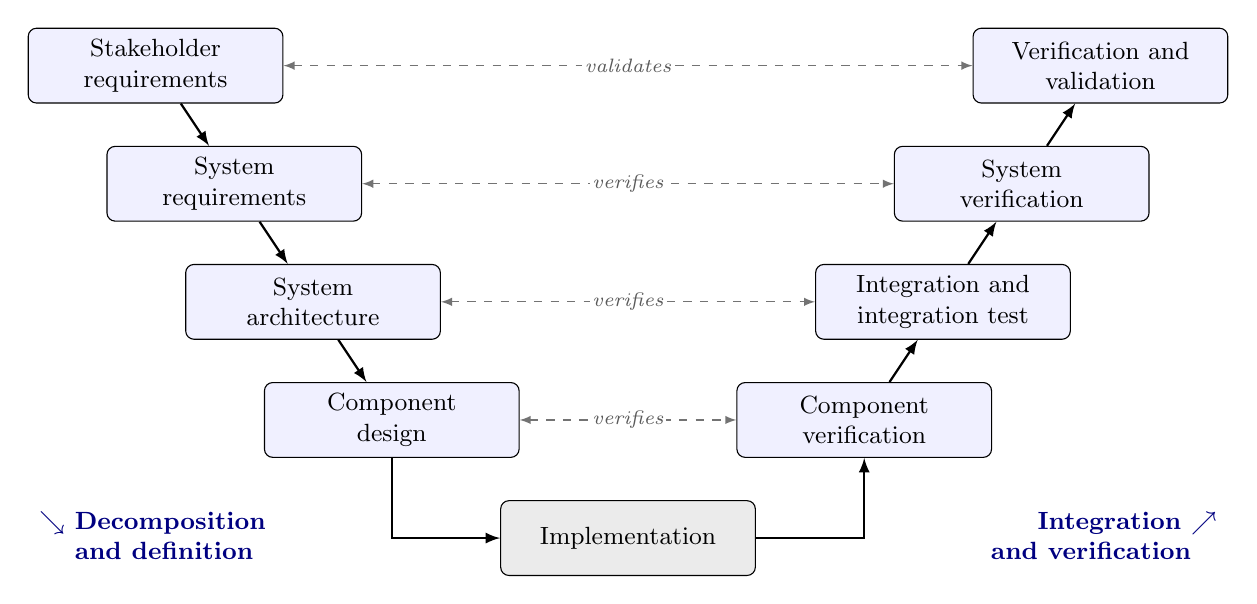
\begin{tikzpicture}[
      >=latex,
      font=\small,
      phase/.style={draw, rounded corners=3pt, fill=blue!6, align=center,
                    minimum width=3.2cm, minimum height=0.95cm, text width=3.0cm},
      impl/.style ={phase, fill=black!8},
      flow/.style ={->, thick},
      link/.style ={<->, dashed, black!55},
      lbl/.style  ={font=\scriptsize\itshape, text=black!65, fill=white, inner sep=1pt},
    ]
    % Left branch: specification and design (top to bottom)
    \node[phase] (req)  at (0.0, 0.0)  {Stakeholder\\requirements};
    \node[phase] (sys)  at (1.0,-1.5)  {System\\requirements};
    \node[phase] (arch) at (2.0,-3.0)  {System\\architecture};
    \node[phase] (comp) at (3.0,-4.5)  {Component\\design};

    % Bottom
    \node[impl]  (impl) at (6.0,-6.0)  {Implementation};

    % Right branch: integration and verification (bottom to top)
    \node[phase] (cver) at (9.0,-4.5)  {Component\\verification};
    \node[phase] (int)  at (10.0,-3.0) {Integration and\\integration test};
    \node[phase] (sver) at (11.0,-1.5) {System\\verification};
    \node[phase] (val)  at (12.0, 0.0) {Verification and\\validation};

    % Process flow along the V
    \draw[flow] (req)  -- (sys);
    \draw[flow] (sys)  -- (arch);
    \draw[flow] (arch) -- (comp);
    \draw[flow] (comp) |- (impl);
    \draw[flow] (impl) -| (cver);
    \draw[flow] (cver) -- (int);
    \draw[flow] (int)  -- (sver);
    \draw[flow] (sver) -- (val);

    % Verification / validation relationships across the V
    \draw[link] (req.east)  -- node[lbl] {validates} (val.west);
    \draw[link] (sys.east)  -- node[lbl] {verifies}  (sver.west);
    \draw[link] (arch.east) -- node[lbl] {verifies}  (int.west);
    \draw[link] (comp.east) -- node[lbl] {verifies}  (cver.west);

    % Branch labels (bottom corners, outside the V)
    \node[font=\small\bfseries, text=blue!50!black, align=left, anchor=west]
      at (-1.6,-6.0) {$\searrow$ Decomposition\\\phantom{$\searrow$} and definition};
    \node[font=\small\bfseries, text=blue!50!black, align=right, anchor=east]
      at (13.6,-6.0) {Integration $\nearrow$\\and verification\phantom{$\nearrow$}};
  \end{tikzpicture}

  \caption[V-model of the system development process]{%
    V-model of the system development process. The left branch decomposes
    stakeholder requirements step by step into system requirements, an
    architecture and component designs; after implementation, the right
    branch integrates the components into the complete system. Each
    level on the right is verified against its counterpart on the left
    (dashed arrows), and the finished system is validated against the
    original stakeholder requirements.}
  \label{fig:vmodel}
\end{figure}
